\documentclass[12pt,a4paper]{article}
\usepackage{amsmath}
\usepackage{amsfonts}
\usepackage{amssymb}
\usepackage{graphicx}
\usepackage{secdot}
\usepackage[left=2cm,right=2cm,top=2cm,bottom=2cm]{geometry}

\author{ Shibayan Biswas, AE21B109\\ Department of Aerospace Engineering\\ IIT Madras\\[3ex] Instructor:\\ \large Professor Dr. Manikandan Mathur}

\title{Experiment- 3}

\date{September 21, 2022}

\begin{document}

\maketitle
\hline
\section{Aim:}
The aim of this particular experiment is to perform the flow-rate measurement of fluid(air) using an orifice.
\section{Introduction:}
An orifice is an opening, of any size or shape, in a pipe or at the bottom or side wall of a container (water tank, reservoir, etc.), through which fluid is discharged. If the geometric properties of the orifice and the inherent properties of the fluid are known, the orifice can be used to measure flow rates. Flow measurement by an orifice is based on the application of Bernoulli’s equation, which states that a relationship exists between the pressure of the fluid and its velocity. The flow velocity and discharge calculated based on the Bernoulli’s equation should be corrected to include the effects of energy loss and viscosity. Therefore, for accurate results, the coefficient of velocity ($C_v$) and the coefficient of discharge ($C_d$) should be calculated for an orifice. This experiment is being conducted to calibrate the coefficients of the given orifices in the lab.
\section{Practical Application:}
Orifices have many applications in engineering practice besides the metering of fluid flow in pipes and reservoirs. Flow entering a culvert or storm drain inlet may act as orifice flow; the bottom outlet of a dam is another example. The coefficients of velocity and discharge are necessary to accurately predict flow rates from orifices.
\section{Objective:}
The objective of this lab experiment is to determine the coefficients of velocity and discharge of two small orifices in the lab and compare them with values in textbooks and other reliable sources.
\section{Method:}
The coefficients of velocity and discharge are determined by measuring the trajectory of a jet issuing fluid from an orifice in the side of a reservoir under steady flow conditions, i.e., a constant reservoir head.
\section{Equipment:}
The following equipment is required to perform the orifice and free jet flow experiment:
\begin{itemize}
\item F1-10 hydraulics bench
\item F1-17 orifice and free jet flow apparatus, with two orifices having diameters of 19 mm and 25 mm
\item Measuring cylinder for flow measurement
\item Stopwatch for timing the flow measurement
\end{itemize}
\begin{figure}[!ht]
	\begin{center}
			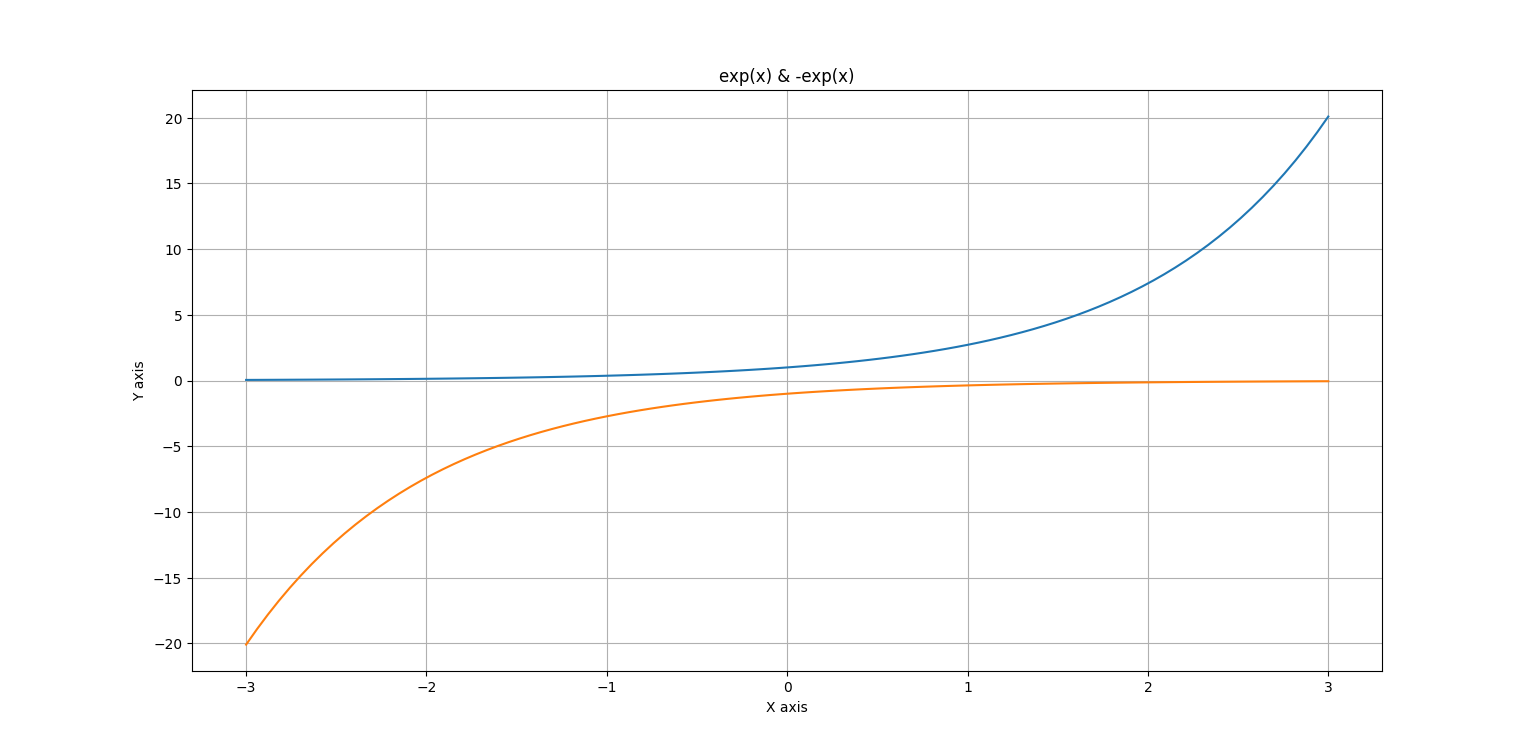
\includegraphics[scale=1.8]{Figure_1.png}
	\end{center}
	\caption{F1-17 Orifice}
\end{figure}
\section{Theory:}
An orifice plate is a thin plate with a hole in it, which is usually placed in a pipe. When a fluid (whether liquid or gaseous) passes through the orifice, its pressure builds up slightly upstream of the orifice but as the fluid is forced to converge to pass through the hole, the velocity increases and the fluid pressure decreases. A little downstream of the orifice the flow reaches its point of maximum convergence, the vena contracta where the velocity reaches its maximum and the pressure reaches its minimum. Beyond that, the flow expands, the velocity falls and the pressure increases. By measuring the difference in fluid pressure across tappings upstream and downstream of the plate, the flow rate can be obtained from Bernoulli's equation using coefficients established from extensive research.\\
\\In the experiment, we will discuss about the topic of “Volumetric flow rate with pressure” and their related facts and their relationship which is applied in the field of engineering. In physics and engineering, in particular fluid dynamics, the volumetric flow rate (also known as volume flow rate, or volume velocity) is the volume of fluid which passes per unit time; usually it is represented by the symbol Q .
The mathematically form of the volumetric flow rate of the piping system is:
\begin{equation}
	\text{Q} = \text{v} \text{A}
\end{equation}
Q = Volumetric flow rate of the liquid substance\\
v = Velocity of the liquid substance\\
A = Cross sectional area of a pipe or a channel\\
\\Also by the definition of pressure we know that pressure is the force applied perpendicular to the surface of an object per unit area over which that force is distributed. Gauge pressure is the pressure relative to the ambient pressure. Various units are used to express pressure. It can be mathematically expressed as:
\begin{equation}
	\text{P} = \frac{\text{F}}{\text{A}}
\end{equation}
P = Pressure\\
F= Net force applied to the pipe or channel\\
A = Cross sectional area\\
\\ Hence we infer from these concepts the relation between volume flow rate and change in pressure that can be mathematically represented as:
\begin{equation}
	\text{q} = \text{$\alpha \epsilon A_d$} \sqrt{\frac{\text{$2 \Delta P$}}{\text{$\rho$}}}
\end{equation}
Q = Volumetric flow rate of the liquid substance\\
$\alpha$ = Flow Restricting Factor\\
$\epsilon$ = Flow Expansion Factor\\
$A_d$ = Area of orifice plate\\
$\Delta P$ = Pressure Drop\\
$\rho$ = Density of Air\\
\clearpage
\begin{figure}[!ht]
	\begin{center}
	    \framebox{
			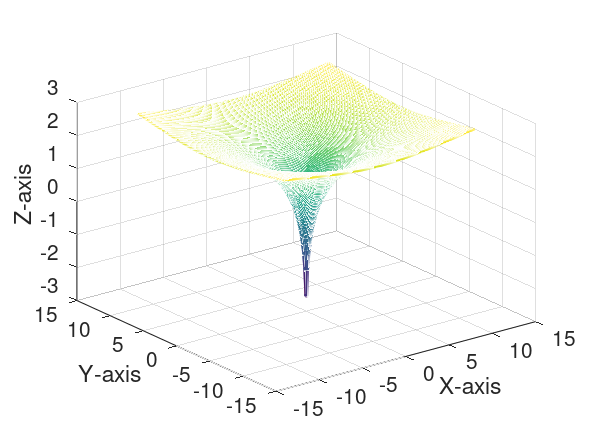
\includegraphics[scale=0.8]{Figure_2.png}
		}
	\end{center}
	\caption{F1-17 Orifice}
\end{figure}
\section{Procedure:}
\begin{itemize}
\item Make sure of every safety measures to minimize the error.
\item Fix the orifice plate of certain diameter.
\item Now turn on compressible flow unit.
\item Note down the corresponding values of velocities and pressure drop shown in manometers.
\item Change the orifice plate diameter and redo the experiment.
\item Determine volume flow rate using velocity.
\item Determine relationship between velocity and pressure drop.
\item Turn off the compressible flow unit.
\end{itemize}
\section{Results:}
The tables representing the experimental and the theoretical values along with the plots showing the variation of the respective values for the following experiment is provided in this section:\\
\\Temperature = 32.6 $^{\circ}$C\\
Density of air = $\rho_{air}$ = 1.164 kg/$m^3$\\
Diameter of Nozzle = 34 mm\\
$\alpha$ for 19 mm Diameter Orifice = 0.64\\
\begin{itemize}
\item When the diameter of the Orifice = 19 mm, we get the following table which represents the values that I have recorded while doing the experiment in the lab and values of the quantities that I have calculated based upon the recorded values.
\begin{table}[h]
\begin{center}
\begin{tabular}{|p{2cm}|p{2.5cm}|p{2cm}|p{2.5cm}|p{2cm}|p{2cm}|}
\hline
Serial No. & Velocity(m/s) & $\Delta P$(KPa) & Q(10^-3$ KPa$) & \sqrt{\Delta P} & $\epsilon$ \\
\hline
1 & 18.58 & 4.9 & 67.4 & 2.21 & 1.01\\
2 & 21.00 & 6.4 & 76.2 & 2.52 & 1.005\\
3 & 24.75 & 9.1 & 89.8 & 3.01 & 0.992\\
4 &2 8.5 & 12.5 & 103.4 & 3.53 & 0.974\\
5 & 31.25 & 15.3 & 113.4 & 3.91 & 0.964\\
\hline
\end{tabular}
\caption{Raw Data Table when Diameter of Orifice = 19 mm}
\end{center}
\end{table}
\begin{itemize}
\item For y = mx + c: m = 6.7489 and c = 2.0058
\item Given: $\alpha$ = 0.64. Therefore, $\epsilon$ = 9947.57, using m = $\alpha \epsilon A_d \sqrt{\frac{\text{$2 \Delta P$}}{\texttt{$\rho$}}}$ 
\end{itemize}
\item When the diameter of the Orifice = 19 mm, we get the following table which represents the values that I have recorded while doing the experiment in the lab and values of the quantities that I have calculated based upon the recorded values.
\begin{table}[h]
\begin{center}
\begin{tabular}{|p{2cm}|p{2.5cm}|p{2cm}|p{2.5cm}|p{2cm}|p{2cm}|}
\hline
Serial No. & Velocity(m/s) & $\Delta P$(KPa) & Q(10^-3$ KPa$) & \sqrt{\Delta P} & $\alpha \epsilon$ \\
\hline
1 & 20.15 & 1.2 & 73.1 & 1.09 & 0.82\\
2 & 26.90 & 2.2 & 97.6 & 1.48 & 0.81\\
3 & 30.00 & 2.8 & 108.8 & 1.67 & 0.80\\
4 & 35.30 & 4.0 & 128.1 & 2.00 & 0.78\\
5 & 40.00 & 5.2 & 145.1 & 2.28 & 0.78\\
\hline
\end{tabular}
\caption{Raw Data Table when Diameter of Orifice = 25 mm}
\end{center}
\end{table}
\begin{itemize}
\item For y = mx + c: m = 15.1741 and c = 1.7710
\item We club the constants together so that $\epsilon$ = $\alpha \epsilon$. Therefore, ε = 6434.35 using m = $\alpha \epsilon A_d \sqrt{\frac{\text{$2 \Delta P$}}{\texttt{$\rho$}}}$
\end{itemize}
\end{itemize}
\\(a) When the diameter of the Orifice is 19 mm:\\
\begin{equation}
\text{$\epsilon$} = \text{0.98}
\end{equation}
\\(b) When the diameter of the Orifice is 25 mm:\\
\begin{equation}
\text{$\alpha \epsilon$} = \text{0.798}
\end{equation}
\clearpage
\begin{figure}[!ht]
	\begin{center}
	    \framebox{
			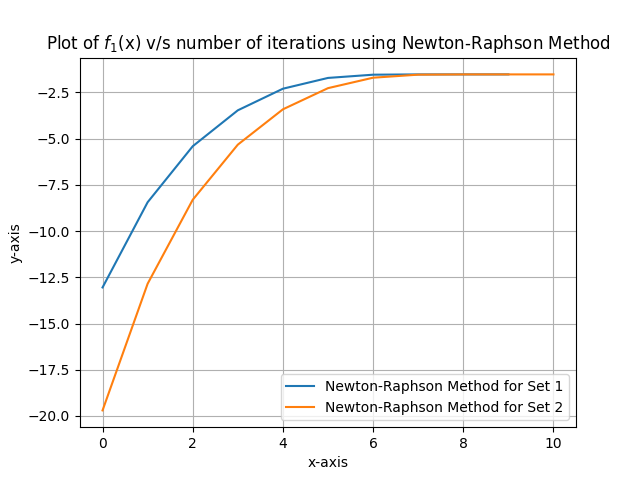
\includegraphics[scale=0.8]{Figure_3.png}
		}
	\end{center}
	\caption{When the diameter of the Orifice Plate = 19 mm}
\end{figure}
\begin{figure}[!ht]
	\begin{center}
	    \framebox{
			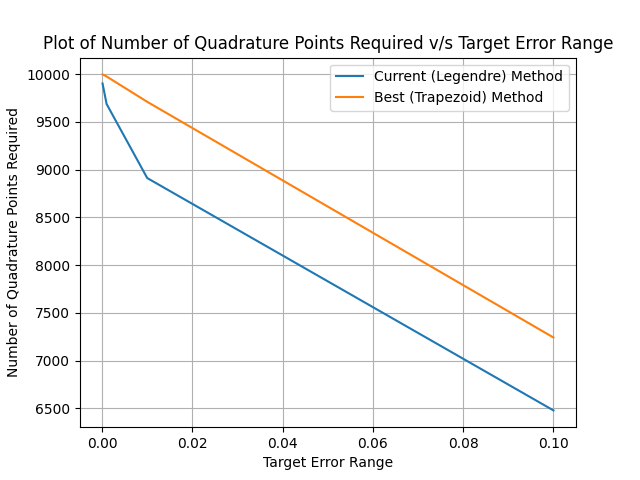
\includegraphics[scale=0.8]{Figure_4.png}
		}
	\end{center}
	\caption{When the diameter of the Orifice Plate = 19 mm}
\end{figure}
\clearpage
\begin{figure}[!ht]
	\begin{center}
	    \framebox{
			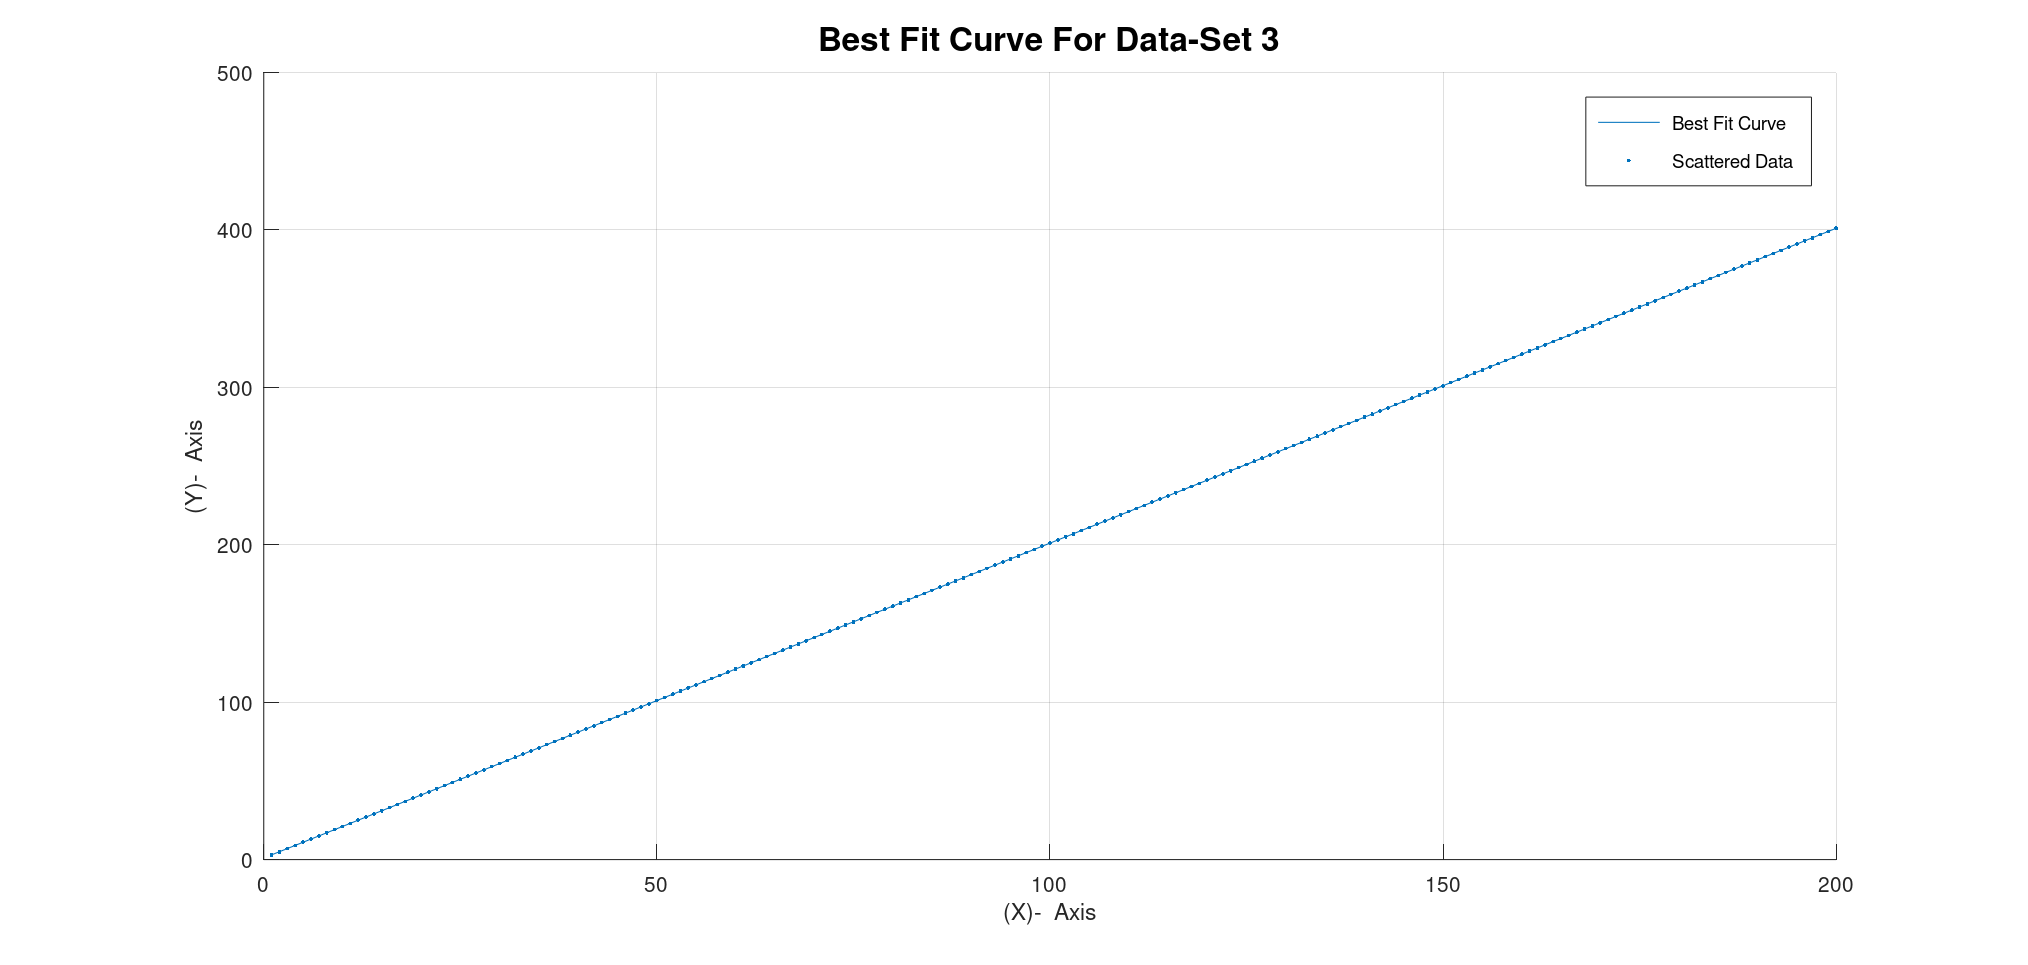
\includegraphics[scale=0.8]{Figure_5.png}
		}
	\end{center}
	\caption{When the diameter of the Orifice Plate = 25 mm}
\end{figure}
\begin{figure}[!ht]
	\begin{center}
	    \framebox{
			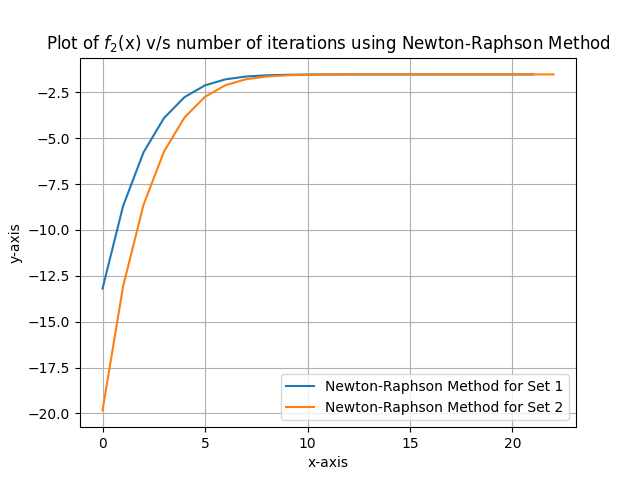
\includegraphics[scale=0.8]{Figure_6.png}
		}
	\end{center}
	\caption{When the diameter of the Orifice Plate = 25 mm}
\end{figure}
\section{Conclusion:}
\begin{itemize}
\item The effects of Viscous Force are not negligible over here.
\item Due to a sudden change in area at the Orifice Plates, the velocity also changes before and after the Orifice Plates.
\item The Volume Flow Rate depends upon the area of cross-section of the Nozzle.
\item The value of $\epsilon$ depends on the ratio of Pressure of the Orifice Plates and the ratio of the Surface Area of the Orifice Plates.
\item The value of $\alpha$ depends on the Reynolds's Number and ratio of the Surface Area of the Orifice Plates.
\item The mathematical relation between Volume Flow Rate and Change in Pressure is valid for Viscous Fluids.
\item From the following experiment we conclude that the Volume Flow Rate is directly proportional to the square root of Change in Pressure.
\end{itemize}
\section{Sources of Error:}
\begin{itemize}
\item The Orifice Plates might not be concentric that can lead to erroneous results.
\item The presence of Viscous Forces can lead to erroneous results.
\item The manometer readings can be sometimes erroneous.
\end{itemize}
\end{document}